
\section{Background}\label{sec:rw}

\subsection{Link between domain modeling and creation of DSLs}
{\bf What are the benefits of DSLs and how does correct modeling relate?}
%Software engineering concerns itself with the science of creating software that is cost-effective, reliable, maintainable and reusable.   Although each criterion is a concern for robotics controllers, the issues of reliability and reusability directly affect engineers' ability to adopt certain toolsets.   

\subsection{Hardware descriptions in existing frameworks}
Many approaches have been used to increase reusability of software artifacts.  Player/Stage drivers can be used directly in ROS \cite{quigley2009}.  Microsoft Robotics Studio uses a service-based paradigm to abstract data sources.  Orocos \cite{Bruyninckx2001} leverages the component design to package related software into a reusable piece.  Carmen \cite{Montemerlo2003}, LCM \cite{Huang2009} and ROS \cite{quigley2009} abstract the message content from the message generation by providing a transport between modules with self-describing data.  These approaches utilize fairly advanced computer science paradigms of distributed development (utilized by many Linux-based open source projects).  Unfamiliarity with these paradigms may discourage many researchers, hobbyists and students from attempting to reuse software, even when it can teach domain specific concepts.

\begin{figure*}[thpb]
      \centering
      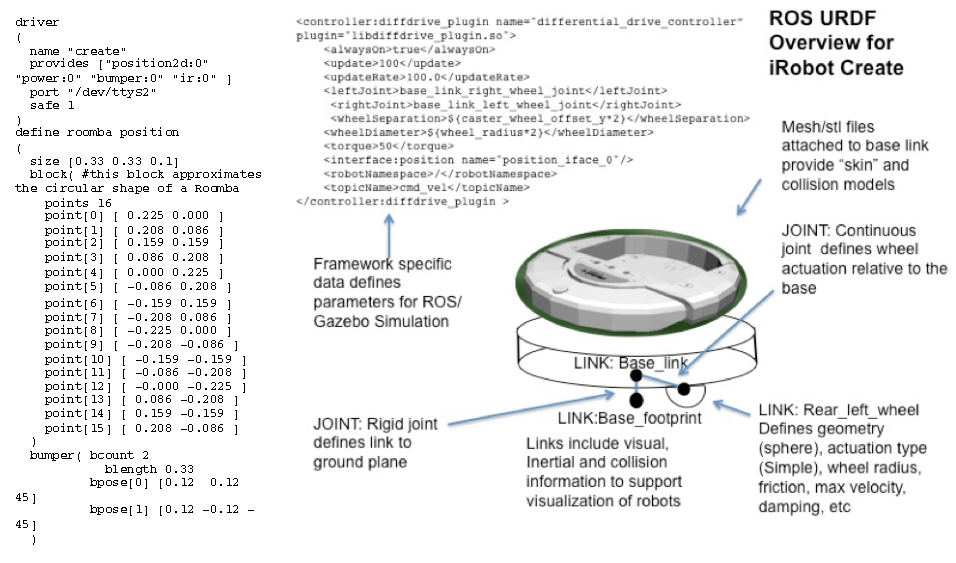
\includegraphics[width=5in]{URDFPS.pdf}
      \caption{Sample device descriptions within frameworks.}
      \label{psurdf}
\end{figure*}

Many frameworks use a declarative description of the robots.  Player/Stage \cite{vaughan2007} is both a 2D simulator and a robot control framework.  Robot description files are broken into two pieces: 1) a 2D description of the robot and its sensors(Figure \ref{psurdf}: right) and 2) a set of interfaces that abstract the data produced by hardware to a standard format.  The description, used for simulating the robot, consists of a polygon-based footprint with sensor locations marked. Actuation and sensor characteristics along with parameters for simplified error models are used to complete the model of the robot.  A domain-specific set of classes and message types describe what data can be obtained or how the robot can be manipulated including position (pose2d) and distance to other objects (single point is range, multipoint is laser).  The classes and message types represent the interface that abstracts the robot hardware to the data that it can produce or consume.  Writing software to the interfaces that a robot can utilize (rather than the specific robot) allows software to be written either for a simulated robot or a real robot, which in turns eases the transition from simulation to physical implementation.

ROS \cite{quigley2009} targets a 3D simulation framework (Gazebo) and more sophisticated intelligent controller, which require a more rigorous description.  UDRF (Uniform Robot Description Format) provides a 3D physical description broken into links and joints to facilitate not only mobile robots but manipulators as well (Figure \ref{psurdf}: right).  Geometric bounding boxes and meshes allow for collision detection and realistic visualization.  Like Player Stage, ROS utilizes a message-based model to decouple data providers from data producers.  Ideally robots that provide and consume similar data types can be controlled similarly.  Unlike Player Stage, URDF not only serves as a mechanism for simulating robots but also allows for the visualization of real robots in both real-time and off-line (through saved messages). 

A select number of robot control frameworks move beyond visualization information and relevant interface declaration in the hardware description.  PREOP, an Alice-based programming interface \cite{cooper2000,wellman2009,anderson2011} for robots takes this paradigm further.  Not only is 3D visualization information supplied but also the programming interface is completely specified by the selection of the robot object.  This is accomplished by linking the real-time control mechanism and exposed API available to the user within the robot object.  

All robotic architectures require that the user provide information regarding the target hardware devices and the resulting data at development time in absentia of the hardware.  Two problems result from this process: 1) users must understand the hardware and resulting data and 2) encode the hardware details properly in the framework of choice.   A mechanism that provides the user with the details of available resources could remove this step and the associated issues with attempting to properly characterize the hardware.  More importantly, hardware that can self-describe could lessen both frustration and the need for in depth hardware knowledge on the part of the user.  

\subsection{RDIS (Robot Device Interface Specification)}
We propose a new paradigm where knowledge of the hardware mechanism is embedded in the hardware, rather than declared in software.  This novel universal design called the (RDIS) Robot Device Interface Specification has three purposes: 1) provide enough information for simulation and visualization of hardware and controllers, 2) declaratively specify the mechanism for requesting data and actuation, and 3) inform users of standard message types that can be obtained from the hardware to facilitate connection to existing frameworks.  The challenge in successfully defining the RDIS is in creating a model that captures the generalizable aspects of robots and provides a mechanism to specialize the aspects that vary.

RDIS (and general reuse in the community) relies upon the relatively invariant nature of mobile robots.  Although some robots are built for a specific task, general use robots within education and research communities tend to leverage designs that provide closed loop inverse kinematic solutions; differential drive being part of this class of robots.  In addition, many robots including the popular Mobile Robots Pioneer class, iRobot Creates, K-Team robots, Erratic ER-1, White Box Robotics Model 914, Ar.Drones, and BirdBrain Finches contain an embedded firmware controller that accepts commands via a serial, Bluetooth, WiFI or USB interface rather than require the users to download a program to onboard memory.  Even robots that require a local software program to run have modes where the local software program presents an API to an external computer (i.e. Lego Mindstorms via Lejos and E-Puck).  In both of these cases, the users create an autonomous controller program that communicates with the firmware to affect actuation and to obtain sensor information.  

%RDIS relies upon two assumptions: 1) robot devices typically contain firmware that manages all hardware resources and exposes access to off-board programs via APIs and 2) many robot devices employ mechanisms that can be generalized and managed at an abstract level.  Not all robot devices contain a firmware that enables off-board programming.  However, this is an assumption that is used within many frameworks (as most frameworks are too processor and memory intensive to run on the limited resources available to on-board controllers).  In addition, firmware often chooses to hide the complexity of managing hardware resources in real time by exposing an API to access and manipulate hardware.

The RDIS specification can be defined as domain specific language (DSL) that is used to program robots at a higher, domain-specific level.  Although the literature reveals very few attempts at using DSLs for hardware device drivers, Thibault et al report the creation of efficient video device drivers using a novel DSL \cite{Thibault1999}.  In the application of robots, the existence of firmware (not programming hardware directly) simplifies the process.  Designing a declarative specification for robot hardware requires a solid domain model of the hardware connection and services that are provided.  Domain models, when designed properly, can be somewhat invariant to changes and can provide a stable basis for deciding the structure and parameters of the specification.  %Figure \ref{circles} shows a typical implementation of mobile robot device driver.  

A preliminary RDIS has been implemented for the Finch robot from Bird Brain and the K-Team Koala\cite{Anderson2012}.  In this design, a JSON-based description file is used (although any syntax can be used including XML).  The intermediate product is an abstract syntax tree that represents the Finch details in a domain specific model.  This intermediate format can be further processed to verify conformance to the specification.  End products are generated from the verified syntax tree, either in a single or multiple passes, using templates that format data based on the model.  The preliminary artifacts generated in this approach   include RDIS specifications and grammars that generate a command line program and a ROS driver.  The ROS driver looks for specific interface signatures that match to ROS message structures.    

